\section{Garments}

We selected four different garments from the Berkeley Garment Library and made
edits to these garment models to create a jacket, a pair of
shorts, a robe, and a vest that fit the size of our human character. The
garments are modeled as a finite element mesh and their motion is
physically simulated
using the ARCSim cloth simulator \cite{Narain:2012:AAR}. We use linear
stretching and bending models and constitutive models derived from
measurements \cite{Wang:2011}. The collisions are detected using a
bounding volume hierarchy \cite{Tang:2010} and resolved with non-rigid
impact zones \cite{Harmon:2008}.

\begin{figure}[!t]
  \centering
  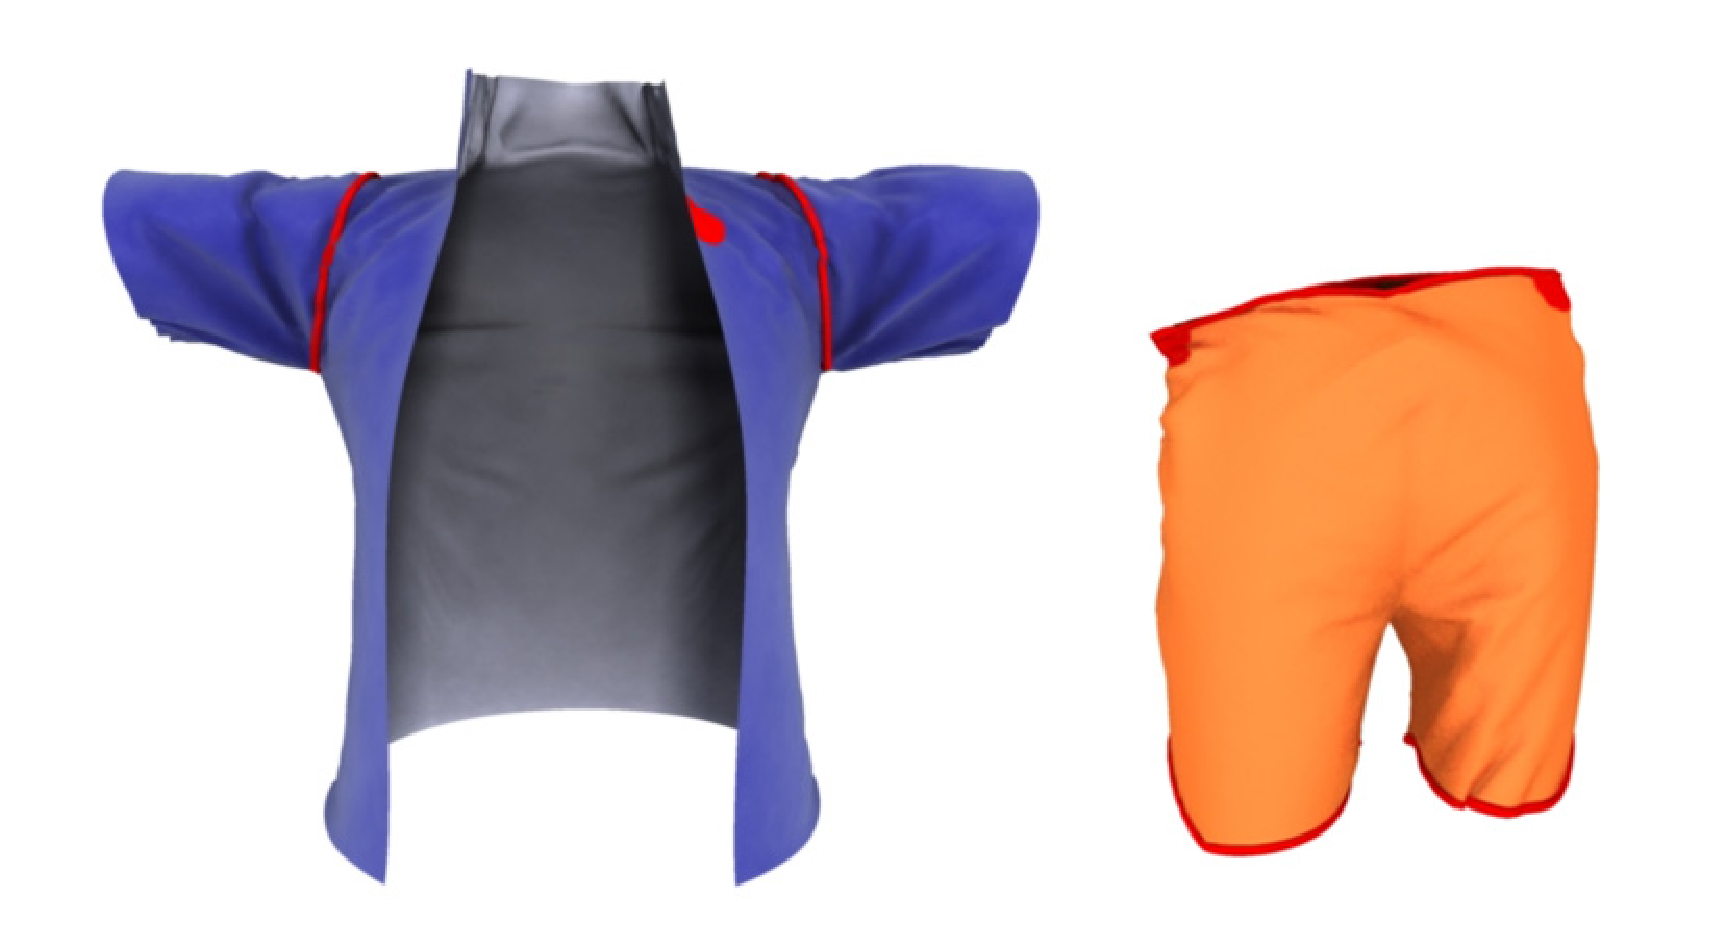
\includegraphics[width=3.5in]{images/features}
  \caption{Cloth features of a jacket and a pair of shorts that are used in dressing control. The red loops and patches are the features for alignment and grip respectively.}
  \label{fig:features}
\end{figure}


\paragraph{Garment Features.} For each garment we defined a set of cloth
features that are important for dressing control. A feature is a set of
vertices on the cloth mesh.  Each feature is either a target for a hand or
foot to align with, or a location for a hand to grasp.  For example, we
use the vertex loop of an armhole as a feature for the hand to target when
putting the arm into a sleeve.  Figure~\ref{fig:feature} shows all the
features that we use for the jacket and the shorts.
